\documentclass[11pt]{article}
\usepackage[a4paper,margin=1in]{geometry}
\usepackage{amsmath,amssymb,amsthm,mathtools,mathrsfs}
\usepackage{graphicx}
\usepackage{microtype}
\usepackage[hidelinks]{hyperref}

\newtheorem{theorem}{Theorem}
\newtheorem{corollary}[theorem]{Corollary}
\newtheorem{lemma}[theorem]{Lemma}
\newcommand{\R}{\mathbb R}
\newcommand{\dist}{\operatorname{dist}}
\newcommand{\domm}{\operatorname{dom}}
\newcommand{\cS}{\mathcal S}

\title{Voronoi stability from quantitative\\flat-direction transversality}
\author{Partial solution packet for arXiv:1212.1094}
\date{11 August 2026}

\begin{document}
\maketitle

\begin{center}
\fbox{\parbox{0.9\linewidth}{\textbf{Candidate partial result.}
Finite-face decomposition can be removed from the source's stability theorem
if cross-site directions stay a positive distance from the directions of flat
segments in the unit sphere.  Closedness of the flat-direction set makes the
source's original qualitative general-position condition sufficient and
covers the cylinder norm in Example 3.5.}}
\end{center}

\section{Source direction and notation}

The source is Daniel Reem, \emph{The geometric stability of Voronoi diagrams
in normed spaces which are not uniformly convex}, arXiv:1212.1094v2
\cite{Reem2013}.  Section 8, PDF page 14, asks in particular to
\begin{quote}
\emph{``weaken the finite face decomposition assumption imposed on the
structure of the unit sphere and to see whether a stability result can be
formulated for the normed spaces induced by the unit spheres mentioned in
Examples 3.4--3.5.''}
\end{quote}

Let $E=(\R^m,\|\cdot\|)$, let $S$ be its unit sphere, and let $X\subset E$ be
compact and convex.  For nonempty sets $P,A\subset X$ with $d(P,A)>0$, define
the symmetric set of normalized cross-directions
\[
 \widehat{P,A}
 =\left\{\pm\frac{a-p}{\|a-p\|}:p\in P,\ a\in A\right\}.
\]
The flat-direction set of the norm is
\[
 \widehat S
 =\left\{\frac{s'-s}{\|s'-s\|}:s\neq s',\ [s,s']\subset S\right\}.
\]
For sites $(P_k)_{k\in K}$, put $A_k=\bigcup_{j\neq k}P_j$ and
\[
 R_k=\domm(P_k,A_k)
 :=\{x\in X:d(x,P_k)\leq d(x,A_k)\}.
\]
The Hausdorff distance is denoted by $D$.

\begin{figure}[p]
\centering
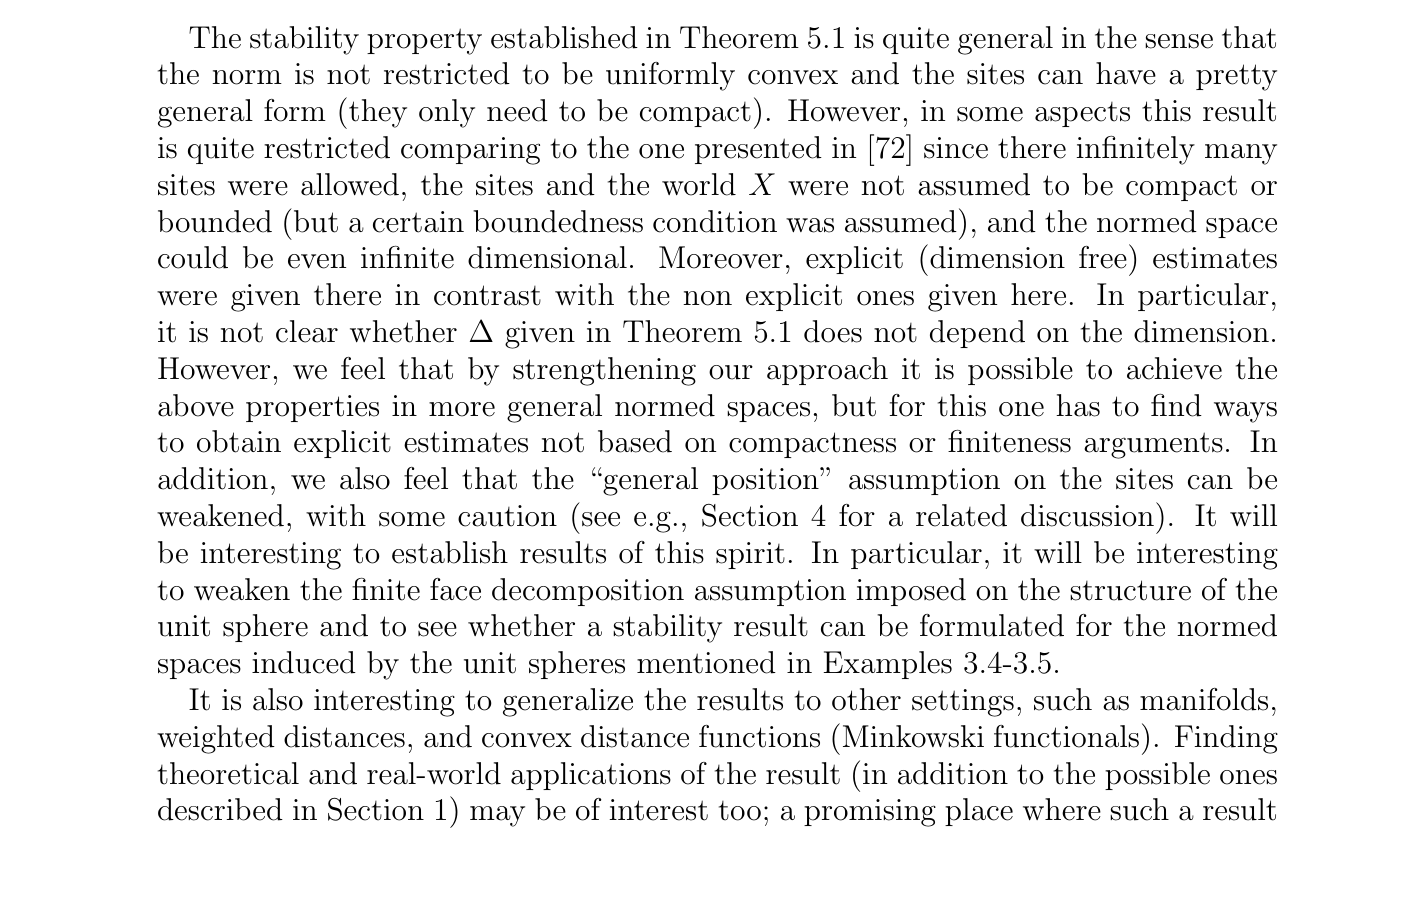
\includegraphics[width=0.96\linewidth]{figures/source_open_direction.png}
\caption{The finite-face weakening direction in Section 8, page 14 of
arXiv:1212.1094v2.}
\end{figure}

\section{Proof intuition}

The source does not use individual faces throughout its long stability proof.
It uses their finiteness once, to turn the qualitative statement ``no site
direction is flat'' into a positive angular separation $2r$.  Everything
after that point is phrased only in terms of $r$.  If the positive separation
is assumed directly, small Hausdorff perturbations move normalized cross-site
directions by at most $4\Delta/\eta$, so half the gap survives.  The source's
uniform-margin lemma then applies simultaneously to the original and
perturbed sites, and its abstract stability proposition finishes the proof.

\section{Stability without finite faces}

\begin{theorem}[quantitative transversality]\label{thm:quant}
Let $X\subset(\R^m,\|\cdot\|)$ be compact and convex, and let
$(P_k)_{k\in K}$ be finitely many nonempty compact sites.  Suppose
\[
 \eta:=\min_{j\neq k}d(P_j,P_k)>0
 \quad\text{and}\quad
 \rho:=\min_{k\in K}\dist(\widehat{P_k,A_k},\widehat S)>0.
\]
Then for every $\epsilon>0$ there is $\Delta>0$ such that, whenever nonempty
compact sites $(P'_k)_{k\in K}$ satisfy
$D(P_k,P'_k)<\Delta$ for every $k$, their Voronoi cells satisfy
\[
 D(R_k,R'_k)<\epsilon\qquad(k\in K).
\]
The corresponding bisectors
$B_k=\{x:d(x,P_k)=d(x,A_k)\}$ satisfy
$D(B_k,B'_k)\leq\epsilon$ after decreasing $\Delta$ if necessary.
No finite-face decomposition of $S$ is assumed.
\end{theorem}

\begin{proof}
We isolate the exact substitution in the source proof.  It is enough to treat
$0<\epsilon<\eta/6$; a smaller tolerance proves any larger one.  Put
$r=\rho/2$ and $M=\operatorname{diam}X$.

The source's Lemma 9.15 states that, for fixed $\epsilon,r>0$, there is a
single $\lambda\in(0,\epsilon)$ giving its radial margin estimate for every
compact pair $(P,A)$ with
\[
 d(P,A)>2\epsilon,
 \qquad \dist(\widehat{P,A},\widehat S)\geq r.
\]
This lemma is proved for an arbitrary finite-dimensional norm and does not use
finite-face decomposition.

Choose $\Delta>0$ so small that
\begin{equation}\label{eq:Delta}
 \Delta<\min\left\{\epsilon,
 \frac{\lambda}{8(1+M/\epsilon)},\frac{r\eta}{8}\right\}.
\end{equation}
For $A'_k=\bigcup_{j\neq k}P'_j$, the elementary union estimate gives
$D(A_k,A'_k)<\Delta$, and hence
\[
 d(P'_k,A'_k)\geq d(P_k,A_k)-2\Delta
 >\eta-2\epsilon>2\epsilon.
\]
The direction estimate in the source's Lemma 9.5 gives
\[
 D(\widehat{P_k,A_k},\widehat{P'_k,A'_k})
 \leq\frac{4\Delta}{\eta}<\frac r2.
\]
Since the original gap is at least $\rho=2r$, the perturbed gap is larger
than $3r/2$, and in particular at least $r$.  Thus Lemma 9.15 supplies the
same radial margin $\lambda$ for all original and perturbed pairs.

The boundedness requirement in the source's Proposition 9.2 holds with
$M=M'=\operatorname{diam}X$.  Its remaining smallness condition is precisely
ensured by the middle term of \eqref{eq:Delta}.  Proposition 9.2 therefore
gives $D(R_k,R'_k)<\epsilon$ for every $k$.

For bisectors, the positive gaps imply the source's no-parallel-segment
condition for both the original and perturbed sites.  Its Theorem 7.1
identifies each bisector with the cell boundary, and the proof of Corollary
5.2 converts the cell estimates just obtained into
$D(B_k,B'_k)\leq\epsilon$.  These arguments also do not use finite faces.
\end{proof}

\section{Qualitative criterion and the cylinder}

\begin{corollary}[closed flat-direction set]\label{cor:closed}
Suppose $\widehat S$ is closed.  Under the other hypotheses of
Theorem~\ref{thm:quant}, assume only the source's qualitative general-position
condition: no segment joining different sites is parallel to a nondegenerate
segment contained in $S$.  Then the conclusions of
Theorem~\ref{thm:quant} hold.

More generally, closedness of $\widehat S$ can be replaced by
\[
 \widehat{P_k,A_k}\cap\overline{\widehat S}=\varnothing
 \qquad(k\in K).
\]
\end{corollary}

\begin{proof}
Because the sites are compact and separated, the map
$(p,a)\mapsto(a-p)/\|a-p\|$ is continuous on each compact product
$P_k\times A_k$.  Hence $\widehat{P_k,A_k}$ is compact.  The qualitative
condition says that it is disjoint from $\widehat S$.  If $\widehat S$ is
closed, compactness of the unit sphere gives positive distance.  The same
argument applies directly with $\overline{\widehat S}$ in the more general
formulation.  Theorem~\ref{thm:quant} now applies.
\end{proof}

\begin{corollary}[cylinder norm]\label{cor:cylinder}
On $E=\R^2\times\R$ equip $(u,z)$ with
\[
 \|(u,z)\|=\max\{\|u\|_2,|z|\}.
\]
For compact separated sites in a compact convex world, Voronoi cells and
bisectors are stable whenever no cross-site segment is horizontal or vertical.
\end{corollary}

\begin{proof}
The unit ball is $B_2\times[-1,1]$.  Any nondegenerate segment in its boundary
lies in a non-singleton exposed face: take a supporting functional at the
midpoint, and linearity forces both endpoints into its maximizing face.

A functional on this product has the form $(v,c)$.  If $v\neq0$ and $c\neq0$,
its maximizing face is a singleton, because the Euclidean disk is strictly
convex and the interval maximum is unique.  If $c=0$, the non-singleton face
is a vertical generator $\{v/\|v\|_2\}\times[-1,1]$; if $v=0$, it is a
horizontal top or bottom disk $B_2\times\{\pm1\}$.  Conversely these faces
contain all vertical and horizontal directions.  Therefore
\[
 \widehat S=\{(u,0):\|u\|_2=1\}\cup\{(0,0,1),(0,0,-1)\},
\]
a closed set.  The stated hypothesis is exactly the source's qualitative
general-position condition, so Corollary~\ref{cor:closed} applies.
\end{proof}

\section{Scope, verification, and novelty}

The theorem gives a stability formulation for arbitrary finite-dimensional
norms, including the source's infinitely faceted examples, provided site
directions avoid the \emph{closure} of the flat directions.  It does not prove
that pointwise avoidance of a nonclosed $\widehat S$ is sufficient; that is the
remaining obstruction for the weakest possible generalization.

A source-level search confirms that finite-face decomposition enters the
proof layer only in Lemmas 9.10 and 9.12, whose downstream output is the gap
used at the first line of the proof of Theorem 5.1.  The constants above were
checked against that proof and Lemmas 9.5 and 9.15.  The packet uses no
computational evidence.  Cheap run indexes and the parsed arXiv corpus found
no later exact theorem under this replacement condition.  Expert review is
recommended, with attention to the dependency audit, preservation of the
direction gap, and the cylinder face classification.  The result is submitted
as a substantial partial answer with moderate novelty confidence.

\begin{thebibliography}{1}
\bibitem{Reem2013}
Daniel Reem,
\newblock \emph{The geometric stability of Voronoi diagrams in normed spaces
which are not uniformly convex},
\newblock arXiv:1212.1094v2, 2013.
\end{thebibliography}

\end{document}
